\chapter{Indicator extractions from event logs}
\label{chapter 4}
\ifpdf
    \graphicspath{{Chapter4/Figs/}{Chapter4/Figs/PDF/}{Chapter4/Figs/}}
\else
    \graphicspath{{Chapter4/Figs/Vector/}{Chapter4/Figs/}}
\fi
The identification and extraction of meaningful process indicators (i.e. Key Process Indicators, KPIs), capable of conveying useful information in a simple, concise, and not misleading way, is a critical challenge in Operations and Process Management. In this chapter, a series of KPIs are proposed as candidates to monitor a manufacturing system: the first section describes what fields are assumed to compose event logs generated by production lines, while the second section explains how event logs are transformed in \textit{case lists}, which are data structures more suitable for the suggested indicator extractions. The last section shows how these KPIs are computed starting from \textit{case lists} and provides a brief description of what they represent.
\section{Assumptions on event logs generated by production lines}
Event logs, as described in section \ref{Event logs}, have a well-defined general-purpose structure, characterized by the association of one row to each event, accompanied by a case identifier and an activity identifier, and also by a variable number of attributes. \\In the particular manufacturing application considered by this thesis, it is assumed that the sensor generated event logs are composed of five fields:
\begin{itemize}
\item \textbf{Event ID}: univocal code of the event. It is assumed that the event order sequence serves as ID of the event. Therefore, Event ID works on an ordinal scale and events are represented with indexes belonging to a set $\Theta$ whose elements are $e\in\{1,2,...,E\}$, where $E$ is number of the events occurring during the process. It is to be noted that, for this application, the information carried by Event ID is redundant, as explained in section \ref{From event logs to case lists}, so this field can be discharged without information loss. 
\item \textbf{Case ID}: univocal code of the job. Since the considered lines are SSLs, with one resource in each stage, and the service policy is BAS, as explained in section \ref{Considered systems}, no case order swap is possible, so the Case ID is equivalent to the job arrival order in the first stage of the line and to the job processing order in each stage. The job arrival order is used as ID for the jobs. Therefore Case ID works on a categorical scale and jobs are represented with indexes belonging to a set $\Gamma$ whose elements are $j\in\{1,2,...,J\}$, where $J$ is the total number of arrived (and processed) jobs in the line. 
\item \textbf{Activity ID}: univocal code of the stage where the event occurs. The definition of activity for the rest of the dissertation is slightly different from the one presented in section \ref{Event logs}: the term activity is not used to indicate a step in the work sequence, but a station in the manufacturing line. Since lines are SSLs, and so stages cannot be concurrent, the occupied position in the line stage sequence is used as identification code of the stage. Therefore, Activity ID works on a categorical scale and stages are represented with indexes belonging to a set $\Sigma$ whose elements are $s\in\{1,2,...,S\}$, where $S$ is the number of stages in the line. 
\item \textbf{Position ID}: univocal code of the position occupied by a sensor in a stage. This ID is univocal only inside a certain stage: multiple sensors in different stages own the same ID if they occupy the same relative position. Position ID works on a categorical scale and positions are represented with indexes belonging to a set $\Pi$ whose elements are $p\in\{1,2,...,P\}$, where $P$ is the number of sensors in each stage, that is three (see section \ref{Considered sensor positions}).
\item \textbf{Timestamp}: instant when the event occurred. This field works on an interval scale, where the zero value is assumed in correspondence with the process starting instant. 
\end{itemize}
\begin{table}[H]
\caption{Example of event log generated by sensors embedded in a production line}
\centering
\label{table:Example of event log}
\scalebox{0.9}{
\begin{tabular}{c c c c c}
  \toprule
  Event ID & Case ID & Activity ID & Position ID & Timestamp \\ 
  \cmidrule{1-5}
  157480 & 7500 & 1 & 1 & 106387.78 \\ 
  157481 & 7500 & 1 & 2 & 106389.37 \\ 
  157482 & 7500 & 1 & 3 & 106392.58 \\ 
  157483 & 7500 & 2 & 1 & 106392.58 \\ 
  157484 & 7500 & 2 & 2 & 106399.19 \\ 
  157485 & 7500 & 2 & 3 & 106413.20 \\ 
  157486 & 7500 & 3 & 1 & 106413.20 \\ 
  157487 & 7500 & 3 & 2 & 106413.20 \\ 
  157488 & 7500 & 3 & 3 & 106416.90 \\ 
  157489 & 7500 & 4 & 1 & 106416.90 \\ 
  157490 & 7500 & 4 & 2 & 106416.90 \\ 
  157491 & 7500 & 4 & 3 & 106423.33 \\ 
  157492 & 7500 & 5 & 1 & 106423.33 \\ 
  157493 & 7500 & 5 & 2 & 106486.05 \\ 
  157494 & 7500 & 5 & 3 & 106498.81 \\ 
  157495 & 7500 & 6 & 1 & 106498.81 \\ 
  157496 & 7500 & 6 & 2 & 106498.81 \\ 
  157497 & 7500 & 6 & 3 & 106506.34 \\ 
  157498 & 7500 & 7 & 1 & 106506.34 \\ 
  157499 & 7500 & 7 & 2 & 106506.34 \\ 
  157500 & 7500 & 7 & 3 & 106513.06 \\ 
  \bottomrule
\end{tabular}
}
\end{table}
Table \ref{table:Example of event log} is provided to show an example of the described field structure, reproducing an event log fragment limited to the trace of a job having CaseID equal to 7500. 
\section{From event logs to case lists}
\label{From event logs to case lists}
Before the indicator extractions, the event log is modified, moving from an event perspective to a case-activity perspective. The datasets obtained modifying event logs are named \textit{case lists}. This conversion is applied to simplify the successive calculations and to organize the data in a structure that better fits the stage-focused study performed through the KPI analysis. \\
A preliminary transformation is the discharge of the Event ID field. Indeed, both Timestamp and Event ID carry the same information (i.e. the event order), however they work on different measurement scales. Timestamp works on an interval scale, while Event ID operates on an ordinal scale. Event ID clearly does not convey any information regarding the time gap between events, just their order of occurrence. Thus, Timestamp is kept, since it is the richer field, and Event ID is dismissed. \\ 
The rest of the event log undergoes a pivoting operation. The Timestamp field is spread in three fields, separating time instants acquired by sensors located in different positions (recorded in Position ID) in the same stage. The resulting fields are named as follows
\begin{itemize}
\item \textbf{Timestamp\_Buffer} ($T_B$): it registers the instant when the job entered in the stage buffer, recorded in event log rows having Position ID equal to 1
\item \textbf{Timestamp\_Resource} ($T_R$): it registers the instant when the job entered in the stage resource, recorded in event log rows having Position ID equal to 2
\item \textbf{Timestamp\_End} ($T_E$): it registers the instant when the resource finished the job processing, recorded in event log rows having Position ID equal to 3
\end{itemize}
\begin{figure}[h] 
\centering    
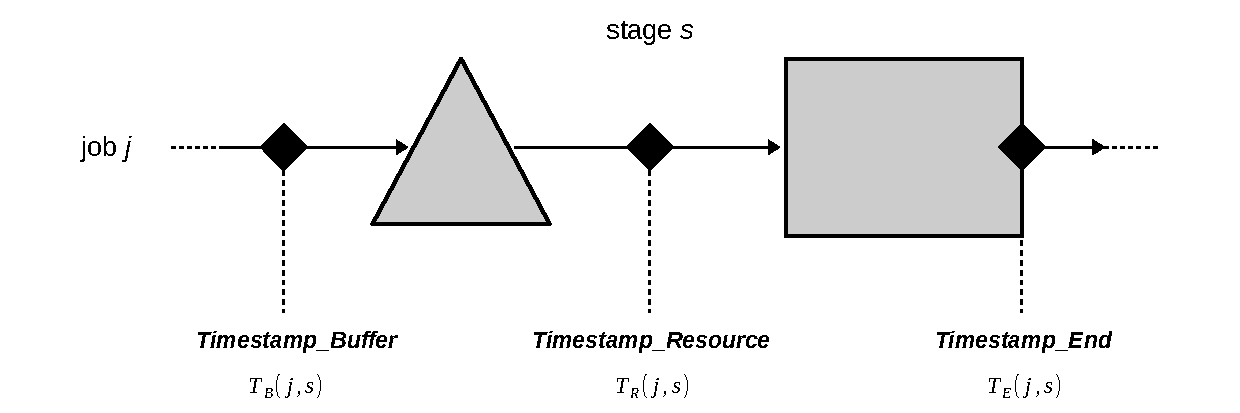
\includegraphics[width=1\textwidth]{Timestamps_thesis}
\caption[Relations between sensors and timestamps]{Relations between sensors and timestamps}
\label{fig:Relations between sensors and timestamps}
\end{figure}
Each row of the resulting dataset records the instants when the sensors in a specific stage observed the passage of a certain job. Each row is uniquely identified by (i.e. the dataset primary key is) the combination of Case ID and Activity ID. \\
For the rest of the thesis, Timestamp fields are going to be referenced as follows
\begin{itemize}
\item $T_B(j,s)$: instant of entrance of job j in the buffer of stage s
\item $T_R(j,s)$: instant of entrance of job j in the resource of stage s
\item $T_E(j,s)$: instant of processing finish of job j in stage s
\end{itemize}
\begin{table}[ht]
\caption{Example of case list}
\centering
\label{table:Example case list}
\scalebox{0.9}{
\begin{tabular}{c c c c c}
  \toprule
  Case ID & Activity ID & Timestamp\_Buffer & Timestamp\_Resource & Timestamp\_End \\ 
  \cmidrule{1-5}
  7500.00 & 1 & 106387.78 & 106389.37 & 106392.58 \\ 
  7500.00 & 2 & 106392.58 & 106399.19 & 106413.20 \\ 
  7500.00 & 3 & 106413.20 & 106413.20 & 106416.90 \\ 
  7500.00 & 4 & 106416.90 & 106416.90 & 106423.33 \\ 
  7500.00 & 5 & 106423.33 & 106486.05 & 106498.81 \\ 
  7500.00 & 6 & 106498.81 & 106498.81 & 106506.34 \\ 
  7500.00 & 7 & 106506.34 & 106506.34 & 106513.06 \\ 
  \bottomrule
\end{tabular}
}
\end{table}
Table \ref{table:Example case list} is provided to show a case list example, computed starting from the event log fragment of table \ref{table:Example of event log}.
\section{Indicator computations}
\label{Indicator computations}
Both basic and derived KPIs are calculated starting from case lists. In this section firstly the basic ones are presented, from which all the others are obtained. Then KPIs calculated aggregating on moving windows are discussed. 
\subsection{Basic KPIs}
\label{Basic KPIs}
These indicators are computed as differences between timestamps, so they are all time intervals (see figure \ref{fig:Basic KPIs scheme}). They are separated in two categories: \textbf{Same Case Intervals} (\textbf{SCI}) KPIs and \textbf{Consecutive Cases Intervals} (\textbf{CCI}) KPIs. The first category includes indicators calculated as differences of timestamps related to a specific job, not necessarily in the same stage. The second category consists of indicators calculated as differences of timestamps related to pairs of jobs consecutively passing in the same sensor position. 
\subsubsection{Same case intervals (SCI) KPIs}
\begin{figure}[H] 
\centering    
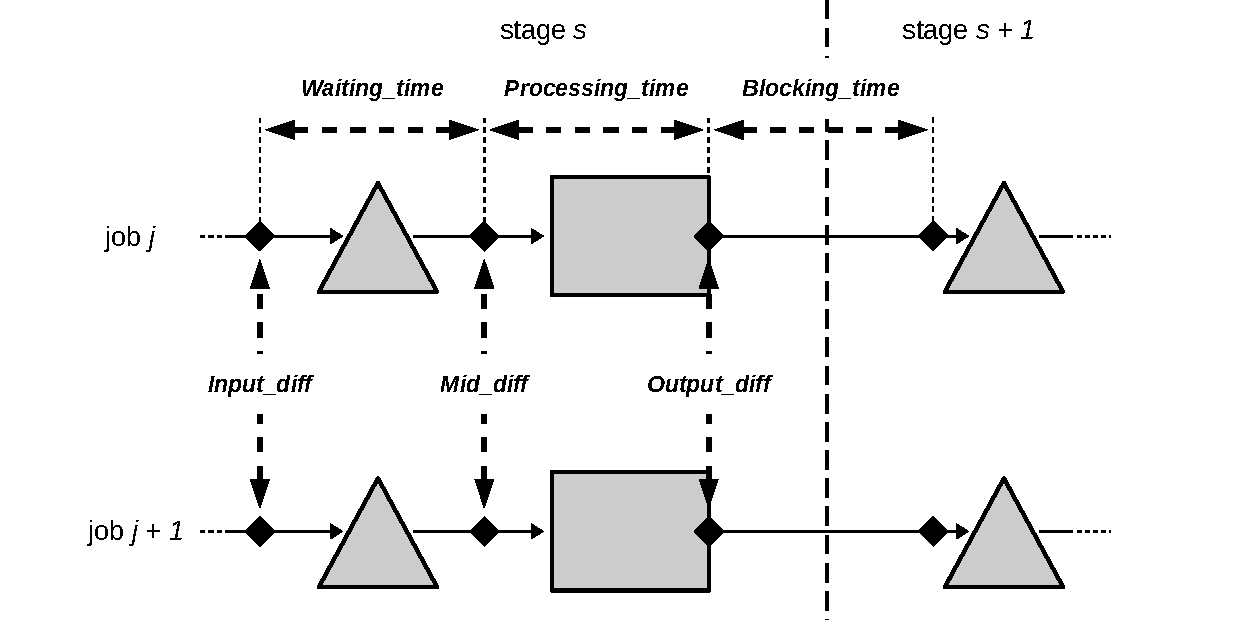
\includegraphics[width=1\textwidth]{Case_intervals_thesis}
\caption[Basic KPI computations scheme]{Basic KPI computations scheme}
\label{fig:Basic KPIs scheme}
\end{figure}
\paragraph{Waiting\_time} is a SCI indicator, computed as the difference between Timestamp\_RESOURCE and Timestamp\_BUFFER (see figure \ref{fig:Waiting time scheme}). Since Timestamp\_BUFFER is the instant when the job entered in the stage buffer, and Timestamp\_RESOURCE  is the instant when the job departed from the buffer and entered in the stage resource, this KPI represents the time spent by a job in a stage buffer. \\
The equation for Waiting\_time of job $j$ in stage $s$ is
\[Waiting\_time(j,s)=T_R(j,s)-T_B(j,s)\]
\begin{figure}[H] 
\centering    

\includegraphics[width=1\textwidth]{Same_case_intervals_WT_thesis}
\caption[Waiting time computation scheme]{Waiting time computation scheme}
\label{fig:Waiting time scheme}
\end{figure}
\paragraph{Processing\_time} is a SCI indicator, computed as the difference between Timestamp\_END and Timestamp\_RESOURCE (see figure \ref{fig:Processing time scheme}). Since Timestamp\_RESOURCE is the instant when the job entered in the stage resource (and started being processed), and Timestamp\_END is the instant when the job processing finished, this KPI represents the time spent by a job in a stage resource while being processed. \\
The equation for Processing\_time of job $j$ in stage $s$ is
\[Processing\_time(j,s)=T_E(j,s)-T_R(j,s)\]
\begin{figure}[H] 
\centering    

\includegraphics[width=1\textwidth]{Same_case_intervals_PT_thesis}
\caption[Processing time computation scheme]{Processing time computation scheme}
\label{fig:Processing time scheme}
\end{figure}
\paragraph{Blocking\_time} is a SCI indicator, computed as the difference between Timestamp\_BUFFER, registered at the entrance of the stage following the considered one, and Timestamp\_END, registered in the considered stage (see figure \ref{fig:Blocking time scheme}). Since Timestamp\_END is the instant when the job ended to be processed by the stage resource, and Timestamp\_BUFFER is the instant when the job entered in the buffer of the following stage, this KPI represents the time spent by a job in a stage resource without being processed; in other words, this is the time interval during which the resource was occupied by the job because the buffer in the following stage was full, causing stage s resource blocking. \\
The equation for Blocking\_time of job $j$ in stage $s$ is
\[Blocking\_time(j,s)=T_B(j,s+1)-T_E(j,s)\]
\begin{figure}[H] 
\centering    

\includegraphics[width=1\textwidth]{Same_case_intervals_BT_thesis}
\caption[Blocking time computation scheme]{Blocking time computation scheme}
\label{fig:Blocking time scheme}
\end{figure}
\subsubsection{Consecutive cases intervals (CCI) KPIs}
\textbf{Input\_diff, Mid\_diff, and Output\_diff} are CCI indicators, computed as the differences between pairs of timestamps\footnote{Input\_diff is related to pairs of Timestamp\_BUFFER, Mid\_diff is related to pairs of Timestamp\_RESOURCE, and Output\_diff is related to pairs of Timestamp\_END} relative to consecutive job passages through the same sensor (see figure \ref{fig:Consecutive cases intervals scheme}). All these KPIs represent time intervals related to the cycle time as perceived by different sensor positions. The values assumed by these indicators during a process in steady state are very similar, as it is going to be shown in subsection \ref{Consecutive cases intervals KPIs - Processing time variation}. \\
The equations for CCI KPIs of job $j$ in stage $s$ are
\[Input\_diff(j,s)=T_B(j+1,s)-T_B(j,s)\]
\[Mid\_diff(j,s)=T_R(j+1,s)-T_R(j,s)\]
\[Output\_diff(j,s)=T_E(j+1,s)-T_E(j,s)\]
\begin{figure}[H] 
\centering    
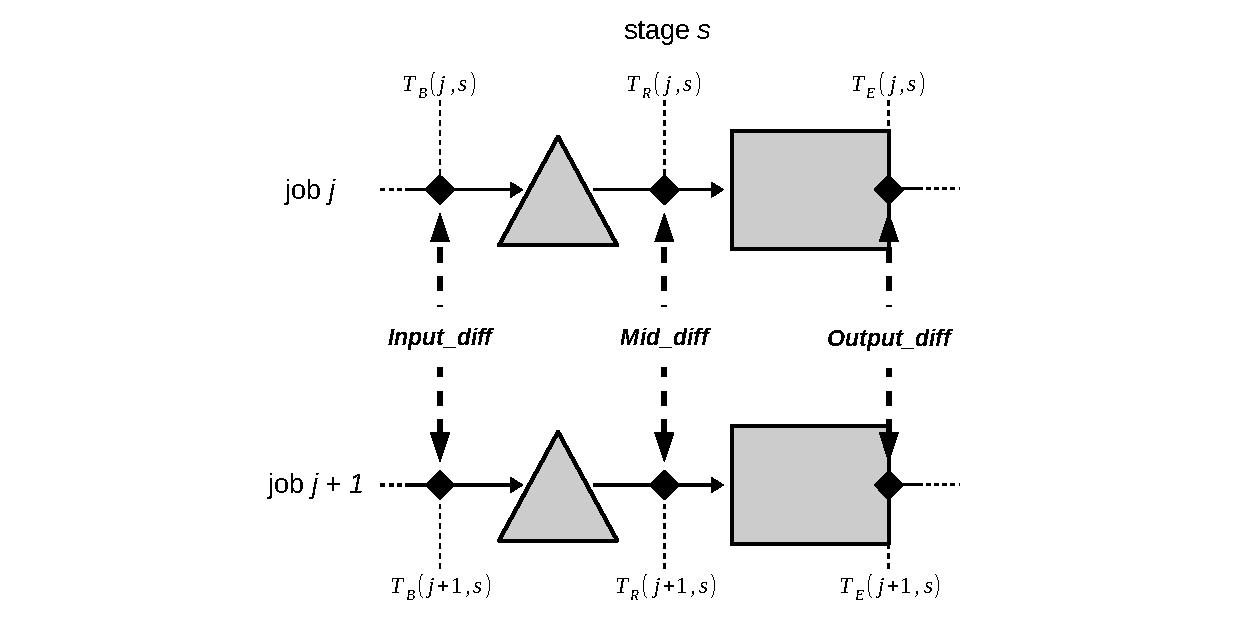
\includegraphics[width=1\textwidth]{Consecutive_cases_intervals_names_thesis}
\caption[Consecutive cases intervals computations scheme]{Consecutive cases intervals computations scheme}
\label{fig:Consecutive cases intervals scheme}
\end{figure}
\subsection{Derived KPIs}
\label{Derived KPIs}
These KPIs are obtained combining the basic KPIs introduced in the previous paragraph. The first indicator belonging to this group is called Starving\_time and it is closely related the SCI KPIs, to such an extent that is considered part of that category for the rest of the dissertation. The other derived KPIs are called Rolling Windows KPIs.
\subsubsection{Starving\_time KPI}
Starving\_time is calculated as the difference between Mid\_diff and the sum of Processing\_time and Blocking\_time (see figure \ref{fig:Starving time scheme}). As said, Mid\_diff represents the time interval between the passages of two consecutive jobs through the same sensor; this means that Mid\_diff cannot be less than Processing\_time (i.e. the time spent by a job being processed), since there is only one resource in each stage and, if the resource is seized, jobs have to wait in the buffer queue. Moreover, Mid\_diff can be greater than Processing\_time for two reasons: first, if the buffer of the following stage is full, a processed job does not release the resource, causing the machine blocking (for a period represented by Blocking\_time) and preventing other jobs to enter in the resource. Second, after a job has released the resource, if the previous buffer is empty, clearly no job seizes the resource, causing starvation. Both these resource statuses contribute to inflate Mid\_diff, that is none other than the sum of these time intervals plus the processing time. Therefore, knowing Mid\_diff, Processing\_time, and Blocking\_time, Starving\_time can be calculated and represents the time interval during which a resource was not working due to lack of jobs in the stage buffer.\\
The equation for Starving\_time of job $j$ in stage $s$ is 
\[Starving\_time(j,s)=Mid\_diff(j,s) - (Processing\_time(j,s)+Blocking\_time(j,s))\]
\begin{figure}[H] 
\centering
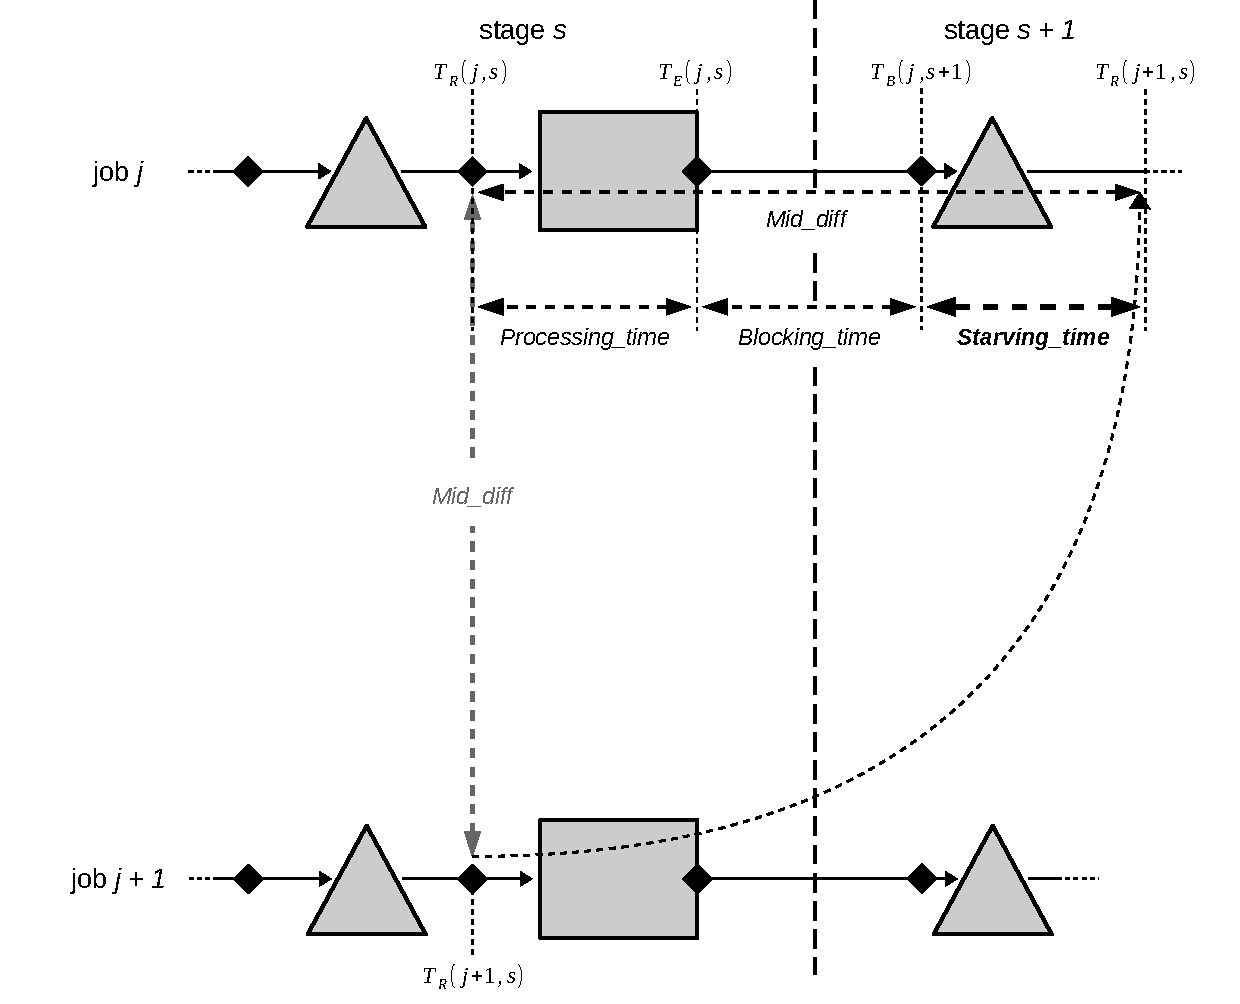
\includegraphics[width=1\textwidth]{Same_case_intervals_ST_thesis}
\caption[Starving time computation scheme]{Starving time computation scheme}
\label{fig:Starving time scheme}
\end{figure}
A more direct, yet less intuitive way to compute this KPI (found simply by replacing the basic indicators with the equations that define them) is differentiating Timestamp\_RESOURCE of the job, immediately following the considered one, entering in the stage resource, and Timestamp\_BUFFER of the considered job entering in the next stage buffer (see figure \ref{fig:Starving time formula visualization}). \\
So, an alternative formula to compute Starving\_time of job $j$ in stage $s$ is
\[Starving\_time(j,s)=T_R(j+1,s)-T_B(j,s+1)\]
\begin{figure}[H] 
\centering    
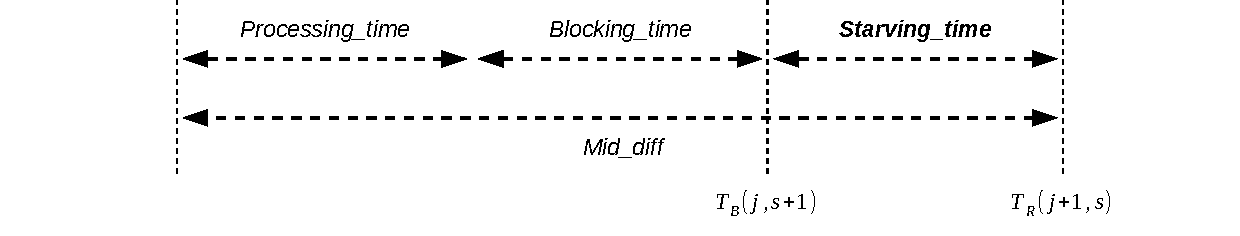
\includegraphics[width=1\textwidth]{Same_case_intervals_ST_scheme}
\caption[Starving time formula visualization]{Starving time alternative formula}
\label{fig:Starving time formula visualization}
\end{figure}
%\subsubsection{Trend KPIs}
%Trend KPIs are calculated as ratios of CCI KPIs (see figure \ref{fig:Trend KPIs scheme}). Since both numerator and denominator are time intervals, these KPIs present as absolute values. They aim to display how the job flow in a specific stage portion behaves over time. 
%\begin{figure}[H] 
%\centering    
%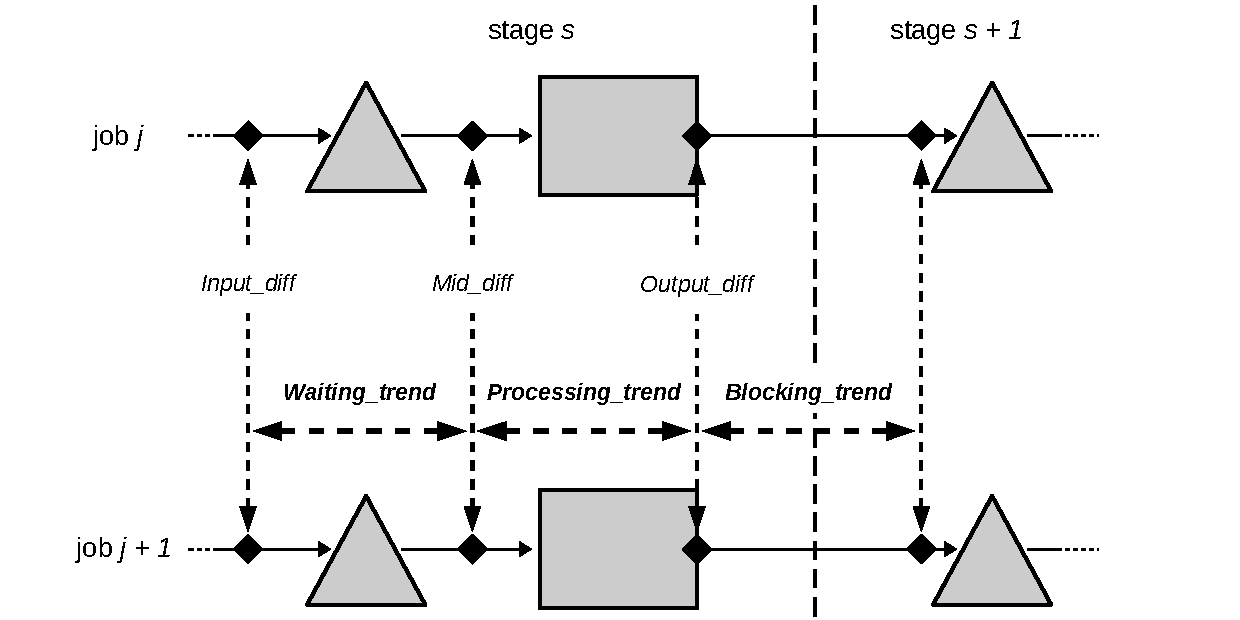
\includegraphics[width=1\textwidth]{Trend_thesis}
%\caption[Trend KPI computations scheme]{Trend KPI computations scheme}
%\label{fig:Trend KPIs scheme}
%\end{figure}
%\paragraph{Waiting\_trend} is computed as the ratio of Mid\_diff and Input\_diff both referring to the same job in the same stage. Since Mid\_diff represents the flow time at a buffer exit, and Input\_diff represents the flow time at a buffer entrance, this KPI shows if the buffer outflow is higher than the inflow or vice versa. Therefore, a greater than one Waiting\_trend (corresponding to a higher outgoing than ingoing flow time, that is a lower outgoing than ingoing flow rate) suggests that the buffer is filling up, whereas a lower than one Waiting\_trend (corresponding to a higher ingoing than outgoing flow time, that is a lower ingoing than outgoing flow rate) suggests that the buffer is emptying.\\
%The equation for Waiting\_trend of job $j$ in stage $s$ is
%\[Waiting\_trend(j,s)=\frac{Mid\_diff(j,s)}{Input\_diff(j,s)}\]
%\paragraph{Processing\_trend} is computed as the ratio of Output\_diff and Mid\_diff referring to the same job in the same stage. Since Output\_diff represents the flow time in correspondence with a job processing finish, and Mid\_diff represents the flow time at a resource entrance, this KPI shows if the resource outflow is higher than the inflow or vice versa. Therefore, a greater than one Processing\_trend (corresponding to a higher outgoing than ingoing flow time, that is a lower outgoing than ingoing flow rate) suggests that the resource is slowing down (i.e. its process capacity is reducing), whereas a lower than one Processing\_trend (corresponding to a higher ingoing than outgoing flow time, that is a lower ingoing than outgoing flow rate) suggests that the resource is accelerating (i.e. its process capacity is increasing).\\
%The equation for Processing\_trend of job $j$ in stage $s$ is
%\[Processing\_trend(j,s)=\frac{Output\_diff(j,s)}{Mid\_diff(j,s)}\]
%\paragraph{Blocking\_trend} is computed as the ratio of Input\_diff of a job in the stage following the considered one, and Output\_diff of the same job in the considered stage. Since Input\_diff represents the flow time at a buffer entrance, and Output\_diff represents the flow time in correspondence with a job processing finish, this KPI shows how blocking affects job flow. Therefore, a greater than one Blocking\_trend suggests that blocking time is increasing (i.e. resource is subject to longer blocking times), whereas a lower than one Blocking\_trend suggests that blocking time is decreasing (i.e. resource is subject to lower blocking times). 
%These indicators are quite useful, even if the carried insights are similar to the ones already offered by corresponding SCI KPIs. Indeed, as [sezione results] shows, these Trend KPIs are steadier and less noise affected, but more reactive to changes than SCI KPIs, resulting suitable to quickly detect variations in the process behavior.\\
%The equation for Blocking\_trend of job $j$ in stage $s$ is
%\[Blocking\_trend(j,s)=\frac{Input\_diff(j,s+1)}{Output\_diff(j,s)}\]
\subsubsection{Rolling Windows KPIs}
Rolling Windows (RW) KPIs are indicators calculated on case list subsection. Since this operation aggregates groups of consecutive rows (i.e. windows) in single records, the resulting dataset has as fewer rows as the subsections are wider. The table containing the aggregation results is named \textit{aggregated case list}. \\ 
RW KPIs are separated in two categories: Moment RW KPIs and Stage Metric RW KPIs. The behavior of this kind of indicators depends on the characteristics of the window which they are computed on. Indeed, windows are characterized by two parameters: length and shift. The length $l$ defines how many rows (i.e. jobs) are included in the dataset subsection. The shift $f$ defines how many rows are between the start of a subsection and the start of the following one, upper extreme included. Windows overlap if shift is lower than length ($f<l$), windows are delayed if shift is higher than length ($f>l$), windows are adjacent if the parameters are equal ($f=l$). Only complete subsections are considered (i.e. all the windows have length $l$, included the first and the last ones), and it is to be noted that the number of windows obtained from a case list varies in function of the windows parameters: the higher the shift and the length, the lower the number of windows obtained from a case list and, therefore, the fewer the rows of the aggregated case list.\\
Since each window includes $l$ jobs, it is conventionally assumed that the Case ID value of the last job $j'$ of a window serves as window ID. So, windows are represented with a set $\Omega$, a subset of set $\Gamma$, whose elements $j'$ depend on window parameters $l$ and $f$, and that includes only indexes of jobs positioned at window ends. So, given certain window parameters values, the elements of set $\Omega$ are defined through the function $j'\in\{l,l+f,l+2f,...\}\subseteq\Gamma$. 
\paragraph{Moment Rolling Windows KPIs} are RW indicators related to moments computed on case list subsections. First order moment (i.e. mean) and second order central moment (i.e. variance) are calculated for each SCI (Starving\_time included), and CCI KPI. \\
These indicators aim to reduce the noise due to process variability, and to concisely display the characteristics of the distributions followed by the related KPIs. \\
The equations for Moment Rolling RW KPIs are
\[Waiting\_time\_MEAN(j',l,f,s)=\text{mean}_j\{Waiting\_time(j,s)\}\]
\[Waiting\_time\_VAR(j',l,f,s)=\text{var}_j\{Waiting\_time(j,s)\}\]

\[Processing\_time\_MEAN(j',l,f,s)=\text{mean}_j\{Processing\_time(j,s)\}\]
\[Processing\_time\_VAR(j',l,f,s)=\text{var}_j\{Processing\_time(j,s)\}\]

\[Blocking\_time\_MEAN(j',l,f,s)=\text{mean}_j\{Blocking\_time(j,s)\}\]
\[Blocking\_time\_VAR(j',l,f,s)=\text{var}_j\{Blocking\_time(j,s)\}\]

\[Starving\_time\_MEAN(j',l,f,s)=\text{mean}_j\{Starving\_time(j,s)\}\]
\[Starving\_time\_VAR(j',l,f,s)=\text{var}_j\{Starving\_time(j,s)\}\]

\[Input\_diff\_MEAN(j',l,f,s)=\text{mean}_j\{Input\_diff(j,s)\}\]
\[Input\_diff\_VAR(j',l,f,s)=\text{var}_j\{Input\_diff(j,s)\}\]

\[Mid\_diff\_MEAN(j',l,f,s)=\text{mean}_j\{Mid\_diff(j,s)\}\]
\[Mid\_diff\_VAR(j',l,f,s)=\text{var}_j\{Mid\_diff(j,s)\}\]

\[Output\_diff\_MEAN(j',l,f,s)=\text{mean}_j\{Output\_diff(j,s)\}\]
\[Output\_diff\_VAR(j',l,f,s)=\text{var}_j\{Output\_diff(j,s)\}\]

\[Waiting\_trend\_MEAN(j',l,f,s)=\text{mean}_j\{Waiting\_trend(j,s)\}\]
\[Waiting\_trend\_VAR(j',l,f,s)=\text{var}_j\{Waiting\_trend(j,s)\}\]

\[Processing\_trend\_MEAN(j',l,f,s)=\text{mean}_j\{Processing\_trend(j,s)\}\]
\[Processing\_trend\_VAR(j',l,f,s)=\text{var}_j\{Processing\_trend(j,s)\}\]

\[Blocking\_trend\_MEAN(j',l,f,s)=\text{mean}_j\{Blocking\_trend(j,s)\}\]
\[Blocking\_trend\_VAR(j',l,f,s)=\text{var}_j\{Blocking\_trend(j,s)\}\]

Each function is computed having 
\[j\in\{j'-l+1,j'-l+2,...,j'\}\wedge j'\in\{l,l+f,l+2f,...\}\]
\paragraph{Stage State Rolling Windows KPIs} are RW indicators that help to monitor buffer and resource, exploiting the flow time to get more insights about their usage. Concerning the buffer, the average number of jobs (in a certain window) in a queue is calculated; then three resource related metrics are computed, that are utilization, probability of blocking, and probability of starvation. All Stage State RW KPIs present the same formula structure, that is the ratio between a SCI derived Moment RW KPI and a CCI derived Moment RW KPI, both calculated on the same dataset subsection. Since both numerator and denominator are time intervals, these KPIs present as absolute values. 
\subparagraph{Average\_Queue} is calculated as the ratio between the Waiting\_time\_MEAN and Input\_diff\_MEAN. Since Waiting\_time\_MEAN is the average time interval spent by jobs waiting in a buffer, and Input\_diff\_MEAN is the average time interval between consecutive jobs entering in a buffer (i.e. average flow time as seen by the buffer), their ratio tells the average number of jobs simultaneously present in a buffer.\\
The equation for Average\_Queue computed in stage $s$ on rolling windows with parameters $l$ and $f$ and having $j'$ as last job is
\[Average\_Queue(j',l,f,s)=\frac{Waiting\_time\_MEAN(j',l,f,s)}{Input\_diff\_MEAN(j',l,f,s)}\]
\subparagraph{Utilization} is calculated as the ratio between the Processing\_time\_MEAN and Mid\_diff\_MEAN. Since Processing\_time\_MEAN is the average time interval needed by a resource to process a job, and Mid\_diff\_MEAN is the average time interval between consecutive jobs entering in a resource (i.e. average flow time as seen by the resource), their ratio tells how much time the resource worked compared to the available time, or, from another point of view, the probability that, in a certain instant, the resource was not idle. \\
The equation for Utilization computed in stage $s$ on rolling windows with parameters $l$ and $f$ and having $j'$ as last job is
\[Utilization(j',l,f,s)=\frac{Processing\_time\_MEAN(j',l,f,s)}{Mid\_diff\_MEAN(j',l,f,s)}\]
\subparagraph{Blocking\_probability} is calculated as the ratio between the Blocking\_time\_MEAN and Mid\_diff\_MEAN. Since Blocking\_time\_MEAN is the average duration of a stop when blocking occurs in a resource, and Mid\_diff\_MEAN is the average time interval between consecutive jobs entering in a resource (i.e. average flow time as seen by the resource), their ratio tells how much time the resource was in a blocking state compared to the available time, or, from another point of view, the probability that, in a certain instant, the resource was blocked. \\
The mathematical equation for Blocking\_probability computed in stage $s$ on rolling windows with parameters $l$ and $f$ and having $j'$ as last job is
\[Blocking\_probability(j',l,f,s)=\frac{Blocking\_time\_MEAN(j',l,f,s)}{Mid\_diff\_MEAN(j',l,f,s)}\]
\subparagraph{Starving\_probability} is calculated as the ratio between the Starving\_time\_MEAN and Mid\_diff\_MEAN. Since Starving\_time\_MEAN is the average time a resource has to wait for the arrival of a new job after being released by the previous one, and Mid\_diff\_MEAN is the average time interval between consecutive jobs entering in a resource (i.e. average flow time as seen by the resource), their ratio tells how much time the resource was in a starving state compared to the available time, or, from another point of view, the probability that, in a certain instant, the resource was starving. \\
The equation for Starving\_probability computed in stage $s$ on rolling windows with parameters $l$ and $f$ and having $j'$ as last job is
\[Starving\_probability(j',l,f,s)=\frac{Starving\_time\_MEAN(j',l,f,s)}{Mid\_diff\_MEAN(j',l,f,s)}\]





